\documentclass{beamer}
\usepackage{../common_slides}

\usepackage{stackengine}
\stackMath
\newlength\matfield
\newlength\tmplength
\def\matscale{1.}
\newcommand\dimbox[3]{%
  \setlength\matfield{\matscale\baselineskip}%
  \setbox0=\hbox{\vphantom{X}\smash{#3}}%
  \setlength{\tmplength}{#1\matfield-\ht0-\dp0}%
  \fboxrule=1pt\fboxsep=-\fboxrule\relax%
  \fbox{\makebox[#2\matfield]{\addstackgap[.5\tmplength]{\box0}}}%
}
\newcommand\raiserows[2]{%
   \setlength\matfield{\matscale\baselineskip}%
   \raisebox{#1\matfield}{#2}%
}
\newcommand\matbox[4]{
  \stackunder{\dimbox{#1}{#2}{$#4$}}{\scriptstyle #3}%
}

\title{Part-of-Speech Tagging \\ + \\ Neural Networks 2}
\date{}
\author{CS 287}
\begin{document}
\maketitle{}

\begin{frame}{Review:  Bilinear Model}
  Bilinear model,
  \[\hat{\boldy} = f((\boldx^0 \boldW^0)\boldW^1 + \boldb)\]
  \begin{itemize}
  \item $\boldx^0 \in \reals^{1 \times d_0}$ start with one-hot.
  \item $\boldW^0 \in \reals^{d_0 \times \din}$, $d_0 = |\mcF|$
  \item $\boldW^1 \in \reals^{\din \times \dout}, \boldb \in \reals^{1 \times \dout}$; model parameters
  \end{itemize}
  \air
  Notes:
  \begin{itemize}
  \item Bilinear parameter interaction.
  \item $d_0 >> \din$, e.g. $d_0 = 10000, \din = 50$
  \end{itemize}

\end{frame}

\begin{frame}{Review:  Bilinear Model: Intuition}
  \[ (\boldx^0 \boldW^0)\boldW^1 + \boldb\]

  
  \[
    \begin{bmatrix}
      0 & \ldots & \textcolor{red}{1} & \ldots & 0 \\
    \end{bmatrix}
    \begin{bmatrix}
      w^0_{1,1} &  \ldots &w^0_{0, \din}\\
      & \vdots & \\
      & \vdots & \\
      & \vdots & \\
      \textcolor{red}{w^0_{k,1}} &  \textcolor{red}{\ldots} &\textcolor{red}{w^0_{k,\din}}\\
      & \vdots & \\
      & \vdots & \\
      & \vdots & \\
      w^0_{d_0, 1} &  \ldots &w^0_{d_0, \din}\\
    \end{bmatrix}
    \begin{bmatrix}
      \textcolor{red}{w^1_{1,1}} &  \ldots & \ldots &   \textcolor{red}{w^1_{0, \dout}}\\
      & \ddots & \ddots &  \\
      \textcolor{red}{w^1_{\din,0}} &  \ldots & \ldots & \textcolor{red}{w^1_{\din, \dout}}\\
    \end{bmatrix}
  \]

\end{frame}

\begin{frame}{Review:  Window Model}
  \textbf{Goal:} predict $t_5$.


  \begin{itemize}
  \item Windowed word model.

  \[ w_1\ w_2\ [\textcolor{red}{w_3\ w_4\ w_5\ w_6\ w_7}]\ w_8 \]

  \item $w_3, w_4$; left context
  \item $w_5$; Word of interest
  \item $w_6, w_7$; right context

  \item $\dwin$; size of window ($\dwin = 5$)
  \end{itemize}
\end{frame}

\begin{frame}{Review: Dense Windowed BoW Features }
  \begin{itemize}
  \item $f_1, \ldots, f_{\dwin}$ are words in window
  \item Input representation is the concatenation of embeddings
  \end{itemize}

  \[ \boldx = [v(f_1)\  v(f_2) \  \ldots \  v(f_{\dwin})]  \]

  Example: Tagging
  \[ w_1\ w_2\ [\textcolor{red}{w_3\ w_4\ w_5\ w_6\ w_7}]\ w_8 \]
  \[ \boldx = [v(w_3)\  v(w_4) \  v(w_5) \ v(w_6) \ v(w_7)]  \]

  \[\renewcommand\matscale{.6}
\matbox{1.5}{4}{\din /5}{} \matbox{1.5}{4}{\din /5}{} \matbox{1.5}{4}{\din /5}{\boldx} \matbox{1.5}{4}{\din /5}{} \matbox{1.5}{4}{\din /5}{}% \raiserows{1.5}{\matbox{4}{2}{d_0}{\dout}{\boldW^0}}  \matbox{4}{2}{\din}{\dout}{\boldW^1} +
% \matbox{7}{2}{1}{\dout}{\boldb}
\]

Rows of $\boldW^1$ encode position specific weights.
\end{frame}


\begin{frame}{Quiz}
  We are doing tagging with a windowed bilinear model with hinge-loss
  and no capitalization features. The model has $\dwin = 5$,
  $\din = 50$, $\dout = 40$, and vocabulary size $10000$.

  \air

  We are given the input window:

  \air


  \begin{center}
    \texttt{The dog walked to the}
  \end{center}

  Unfortunately we incorrectly classify \texttt{walked} as \texttt{NN}
  as opposed to \texttt{VP}, in a bilinear model with a hinge-loss .
  \air


  What is the maximum number of parameters that
  receive a non-zero gradient?
\end{frame}


\begin{frame}{Answer: }
  \begin{center}





      
  \[{\tiny
    \begin{bmatrix}
       \textcolor{red}{1}   & \textcolor{red}{1} &  \textcolor{red}{1} &
 \textcolor{red}{1}  & \textcolor{red}{1} \\
    \end{bmatrix}
    \begin{bmatrix}
      w^0_{1,1} &  \ldots &w^0_{0, \din}\\
      \textcolor{red}{w^0_{the,1}} &  \textcolor{red}{\ldots} &\textcolor{red}{w^0_{the,\din}}\\
      \vdots \\
      \textcolor{red}{w^0_{dog,1}} &  \textcolor{red}{\ldots} &\textcolor{red}{w^0_{dog,\din}}\\
      \vdots \\
      \textcolor{red}{w^0_{walked,1}} &  \textcolor{red}{\ldots} &\textcolor{red}{w^0_{walked,\din}}\\
      \vdots \\
      \textcolor{red}{w^0_{to,1}} &  \textcolor{red}{\ldots} &\textcolor{red}{w^0_{to,\din}}\\
      \vdots \\
      \textcolor{red}{w^0_{the,1}} &  \textcolor{red}{\ldots} &\textcolor{red}{w^0_{the,\din}}\\
      \vdots \\
      w^0_{d_0, 1} &  \ldots &w^0_{d_0, \din}\\
    \end{bmatrix}
    \begin{bmatrix}
      w^1_{1,1} &  \ldots&  \textcolor{red}{w^1_{1,NN}} & \ldots &  \textcolor{red}{w^1_{1,VP}} &    w^1_{0, \dout}\\
                & \ddots & \ddots &                    &         &                                   &  \\
      w^1_{\din,0} &  \ldots&  \textcolor{red}{w^1_{\din,NN}} & \ldots &  \textcolor{red}{w^1_{\din,VP}} &  w^1_{\din, \dout}\\
    \end{bmatrix}
    }
  \]



\air

  $\boldW^0 = 5 \times \din$

  $\boldW^1 = \din \times 2$
  \end{center}

\end{frame}


\begin{frame}{Part-of-Speech Tagging}
  Consider the following windowed model, and 
  assume for now a linear model.

  \[w_1\ \mathrm{\texttt{the}}\ w_3\ w_4\ w_5\] 
  

  \begin{itemize}
  \item What information do we have about the tag of $w_3$?
    \air 

  \item What weight should the features values associated with
    \texttt{the} in position $w_2$ take?
  \end{itemize}
\end{frame}

\begin{frame}{Part-of-Speech Tagging}
  Next Consider the following windowed model, and 
  assume for now a linear model.

  \[w_1\ w_2 \ w_3\ \mathrm{\texttt{dog}} \ w_5\] 
  

  \begin{itemize}
  \item What information do we have about the tag of $w_3$?
    \air 

  \item What weight should the features values associated with
    \texttt{dog} in position $w_4$ take?
  \end{itemize}

\end{frame}


\begin{frame}{Part-of-Speech Tagging}
  Now finally consider the following windowed model, and 
  assume for now a linear model.

  \[w_1\ \texttt{the} \ w_3\ \mathrm{\texttt{dog}} \ w_5\] 
  

  \begin{itemize}
  \item What information do we have about the tag of $w_3$?
    \air 

  \item What weight would we want if we combined both the features values?
  \end{itemize}

\end{frame}

\begin{frame}{Table}
  
\end{frame}

\section{Neural Networks}

\begin{frame}
  \begin{center}
    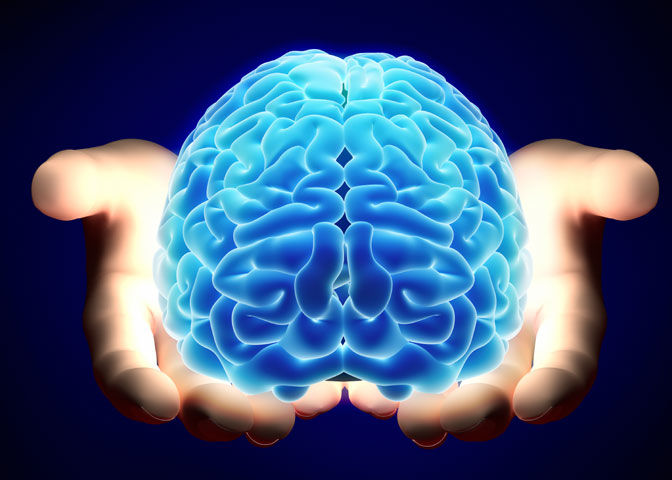
\includegraphics[width=5cm]{brain}
  \end{center}
\end{frame}


\begin{frame}{Neural Network}
  One-layer multi-layer perceptron architecture,

  \[NN_{MLP1}(\boldx) =  g(\boldx\boldW^1 + \boldb^1)W^2 + \boldb^2\]
  \begin{itemize}
  \item $\boldx\boldW + \boldb$; \textit{perceptron}
  \item $\boldx$ is the dense representation in $\reals^{1 \times \din}$
  \item $\boldW^1 \in \reals^{\din \times \dhid}, \boldb^1 \in \reals^{1 \times \dhid}$; first affine transformation
  \item $\boldW^2 \in \reals^{\dhid \times \dout}, \boldb^2 \in \reals^{1 \times \dout}$; second affine transformation
  \item $g:\reals^{\dhid \times \dhid}$ is an \textit{activation non-linearity} (often pointwise)
  \item $g(\boldx\boldW^1 + \boldb^1)$ is the \textit{hidden layer}
  \end{itemize}
\end{frame}

\begin{frame}{Schematic}
  \begin{center}
    

  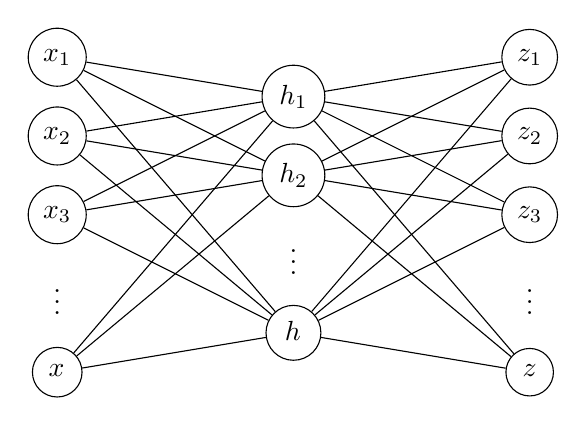
\begin{tikzpicture}
    \node(aa)[draw, circle]{$x_1$};
    \node(ab)[below of =  aa, draw, circle]{$x_2$};
    \node(ac)[below of = ab, draw,circle]{$x_3$};
    \node(ad)[below of = ac]{$\vdots$};
    \node(ae)[below of =  ad, draw, circle]{$x_{\din}$};


    \node(ba)[xshift= 2cm, yshift=-0.5cm, right of = aa, draw, circle]{$h_1$};
    \node(bb)[below of =  ba, draw, circle]{$h_2$};
    \node(bc)[below of = bb]{$\vdots$};

    \node(bd)[below of =  bc, draw, circle]{$h_{\dhid}$};

    \path[draw] (aa) -- (ba); 
    \path[draw] (aa) -- (bb); 
    \path[draw] (aa) -- (bd); 

    \path[draw] (ab) -- (ba); 
    \path[draw] (ab) -- (bb); 
    \path[draw] (ab) -- (bd); 

    \path[draw] (ac) -- (ba); 
    \path[draw] (ac) -- (bb); 
    \path[draw] (ac) -- (bd); 

    \path[draw] (ae) -- (ba); 
    \path[draw] (ae) -- (bb); 
    \path[draw] (ae) -- (bd); 


    \node(ca)[xshift= 2cm, yshift=0.5cm, right of = ba, draw, circle]{$z_1$};
    \node(cb)[below of =  ca, draw, circle]{$z_2$};
    \node(cc)[below of =  cb, draw, circle]{$z_3$};
    \node(cd)[below of = cc]{$\vdots$};
    \node(ce)[below of =  cd, draw, circle]{$z_{\dout}$};


    \path[draw] (ba) -- (ca); 
    \path[draw] (ba) -- (cb); 
    \path[draw] (ba) -- (cc); 
    \path[draw] (ba) -- (ce); 

    \path[draw] (bb) -- (ca); 
    \path[draw] (bb) -- (cb); 
    \path[draw] (bb) -- (cc); 
    \path[draw] (bb) -- (ce); 

    \path[draw] (bd) -- (ca); 
    \path[draw] (bd) -- (cb); 
    \path[draw] (bd) -- (cc); 
    \path[draw] (bd) -- (ce); 


  \end{tikzpicture}  
  \end{center}
\end{frame}

\begin{frame}{Non-Linear Functions}
  Logistic sigmoid function:
  \[\sigma(t) = \frac{1}{1 + \exp(-t)} \]
  \begin{figure}
    \centering
    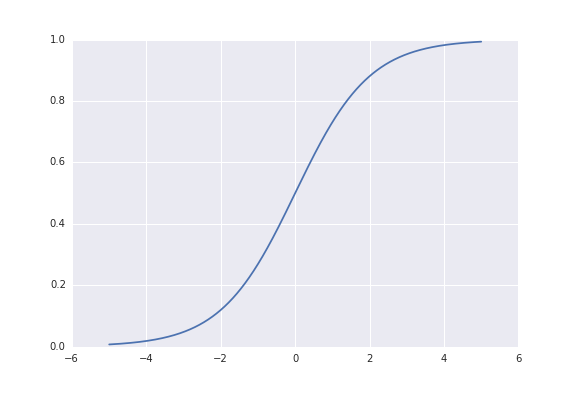
\includegraphics[width=5cm]{../notebooks/sigmoid}
  \end{figure}

  \begin{itemize}
  \item $\sigma((\boldx\boldW^1 + \boldb^1)_i)$
  \item Intuition: Each hidden dimension (``neuron'') is result of logistic regression.
  \item These probabilities are ``features'' for next layer. 
  \end{itemize}
\end{frame}

\begin{frame}{Feature Conjunctions}
  Consider the example ... 
\end{frame}


\begin{frame}{Non-Convexity}

  \begin{itemize}
  \item 
  \end{itemize}
\end{frame}


\begin{frame}
  Why are these better?
\end{frame}


\begin{frame}{Other Non-Linearities: ReLU}
  Rectified Linear Unit:
  \begin{figure}
    \centering
    \[\relu(t) = \max\{0, t\} \]
    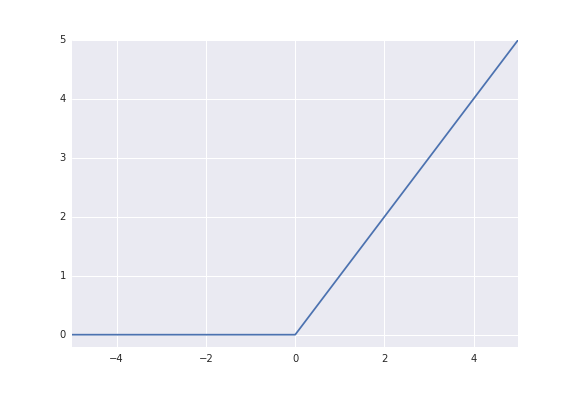
\includegraphics[width=5cm]{../notebooks/Relu}
  \end{figure}
  Intuition:
\end{frame}


\begin{frame}{Saturation}
  
\end{frame}


\begin{frame}{Saturation: Intuition}
  
\end{frame}


\begin{frame}
    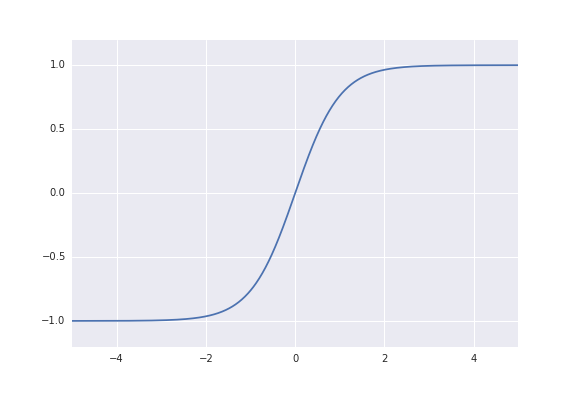
\includegraphics[width=5cm]{../notebooks/tanh}
\end{frame}



\begin{frame}{Function Approximator}
  MLP1 is a universal approximator
\end{frame}

\begin{frame}{Deep Neural Networks (DNNs)}

  Can stack MLPs, 

  \[NN_{MLP1}(\boldx) =  g(\boldx\boldW^1 + \boldb^1)W^2 + \boldb^2\]
  \[NN_{MLP2}(\boldx) =  g(NN_{MLP1}(\boldx) \boldW^1 + \boldb^1)W^2 + \boldb^2\]

  \begin{itemize}
  \item Can have multiple hidden layers, etc.
  \end{itemize}
\end{frame}


\begin{frame}{Other types of networks}
  Highway Network (one example)
  \[NN_{MLP2}(\boldx) =  g(NN_{MLP1}(\boldx) \boldW^1 + \boldb^1)W^2 + \boldb^2\]

\end{frame}


\begin{frame}{Deep Neural Networks (DNNs)}
  
\end{frame}

\section{Backpropagation}

\begin{frame}
  Consider a vector-valued parameterized function  $f(\boldx;\boldtheta)$ where 
  
  \begin{itemize}
  \item $f(\boldx): \reals^m \mapsto \reals^n$; function
  \item $\boldtheta \in \reals^d$; function parameters 
  \end{itemize}
\end{frame}


\begin{frame}
  Consider a scalar-valued loss function  $L(\boldx;\boldtheta)$ where 
  
  \begin{itemize}
  \item $L(\boldx): \reals^n \mapsto \reals$; function
  \end{itemize}
\end{frame}

\begin{frame}{Backpropagation}
  Forward 
  Compute $L(f(\ldots f()))$


  Backward   

  \[ \frac{\partial L}{\partial f(\ldots f(x_i))  } = \sum_{j =1}^m \frac{\partial f(\boldx)_j} {\partial  x_i} \frac{\partial L(f(\boldx))} {\partial f(\boldx)_j}   \]
\end{frame}

\begin{frame}{Torch Implementation}
  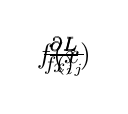
\begin{tikzpicture}
    \node{$\boldx$};
    \node{$\frac{\partial L}{x_i}$};
    \node{$\frac{\partial L}{f(\boldx)_j}$};
    \node{$f(x)$};

  \end{tikzpicture}
    $\frac{\partial L}{\boldtheta_k}$
    $\boldtheta$
\end{frame}

\begin{frame}{Torch Implementation}
  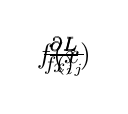
\begin{tikzpicture}
    \node{$\boldx$};
    \node{$\frac{\partial L}{x_i}$};
    \node{$\frac{\partial L}{f(\boldx)_j}$};
    \node{$f(x)$};

  \end{tikzpicture}
    $\frac{\partial L}{\boldtheta_k}$
    $\boldtheta$
\end{frame}

\begin{frame}{Torch Names}

  \begin{itemize}
  \item $\boldx$; \textit{input}
  \item $f(\boldx)$; \textit{self.output} (saved on forward pass)
  \item $\frac{\partial L}{x_i}$; \textit{self.gradInput}
  \item $\frac{\partial L}{f(\boldx)_j}$; \textit{gradOutput}
  \item $\boldtheta$; \textit{gradWeight}
  \item $\frac{\partial L}{\boldtheta}$; \textit{gradWeight}
  \end{itemize}
\end{frame}

\begin{frame}{Max}
  
\end{frame}


\begin{frame}{Max}
  
\end{frame}

\section{Semi-Supervised Training}

\begin{frame}

\end{frame}

\end{document}